\chapter{Search for boosted low mass resonances in the $b\bar{b}$ final state}\label{chapter:analysis}

\begin{figure}[htbp]
 \centering
 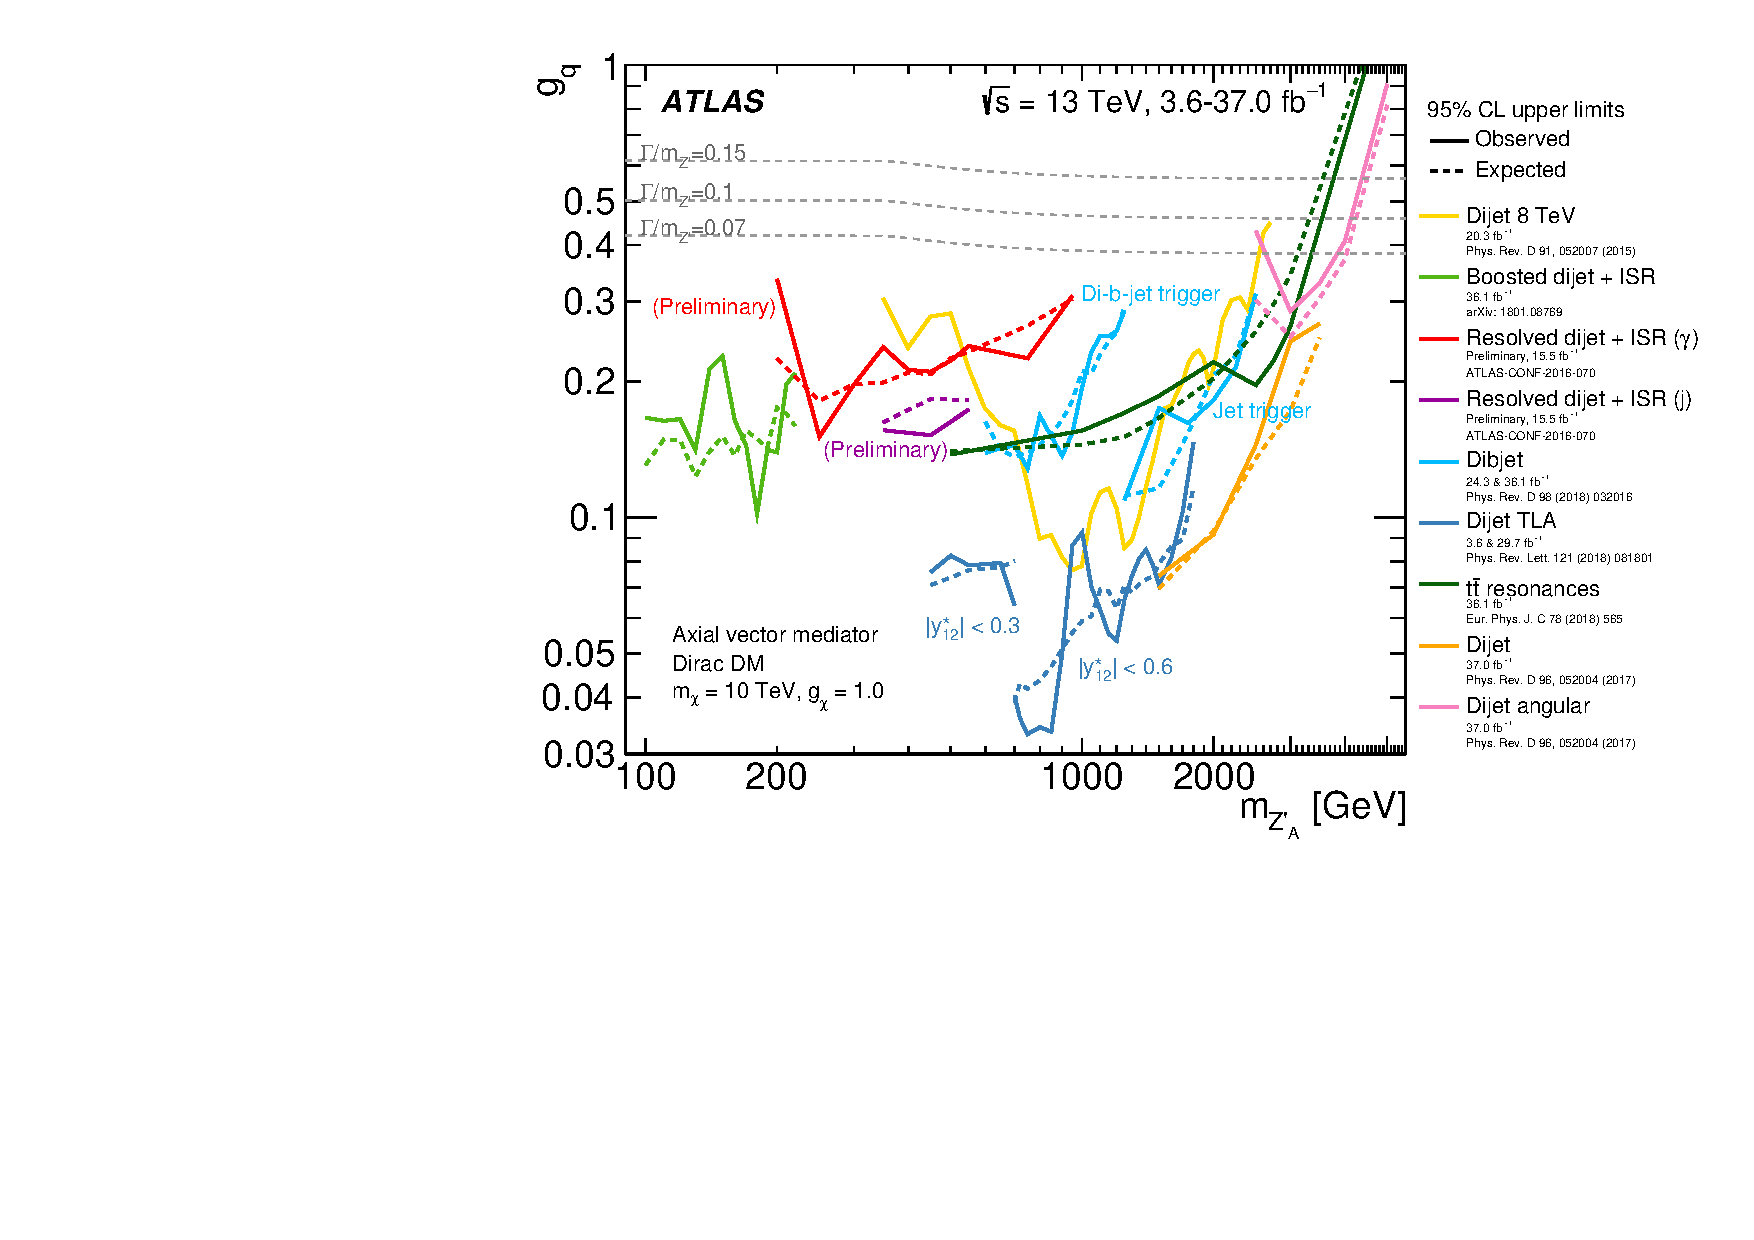
\includegraphics[width=\linewidth]{analysis/darkmatter_coupling_summary.pdf}
 \caption[Dijet search contours for $95\%$ CL upper limits on the coupling $g_{q}$ for the leptophobic axial-vector $Z'_{A}$ model.]{%
 Dijet search contours for $95\%$ CL upper limits on the coupling $g_{q}$ as a function of the resonance mass $m_{Z'_{A}}$ for the leptophobic axial-vector $Z'_{A}$ model.
 The expected limits from each search are indicated by dotted lines.
 The TLA dijet analysis has two parts, employing different datasets with different selections in the rapidity difference $y^{*}$ as indicated.
 The yellow contour shows the results of the dijet search using $20.3~\mathrm{fb}^{-1}$ of $8~\TeV$ data.
 Coupling values above the solid lines are excluded, as long as the signals are narrow enough to be detected using these searches.
 The TLA dijet search with $\abs{y^{*}} < 0.6$ is sensitive up to $\Gamma/m_{Z'} = 7\%$, the TLA dijet with $\abs{y^{*}} < 0.3$ and dijet + ISR searches are sensitive up to $\Gamma/m_{Z'} = 10\%$, and the dijet and dibjet searches are sensitive up to $\Gamma/m_{Z'} = 15\%$.
 The dijet angular analysis is sensitive up to $\Gamma/m_{Z'} = 50\%$.
 No limitation in sensitivity arises from large width resonances in the $t\bar{t}$ resonance analysis.
 Benchmark width lines are indicated in the canvas.
 The $\Gamma/m_{Z'} = 50\%$ lies beyond the canvas borders~\cite{EXOT-2017-32}.}
 \label{fig:darkmatter_coupling_summary}
\end{figure}

\section{Systematic Uncertainties}\label{sec:systematic_uncertainties}

The impact of a systematic uncertainty is defined as the difference in quadrature between the uncertainty in $\mu$ computed when all other uncertainties are considered and when they are fixed to their pre-fit values.
The total systematic uncertainty is then defined as the difference in quadrature between the total uncertainty in $\mu$ and the total statistical uncertainty~\cite{ATLAS-CONF-2018-052}.
The systematic uncertainties and their impacts on the measurement of the signal strengths are summarized in \Cref{table:systematic_uncertainties}.

\begin{table}[htpb]
 \centering
 \caption[Summary of the impact of the main systematic uncertainties on the signal strength uncertainties.]{%
  Summary of the impact $(\sqrt{\Delta \sigma^2}/\mu)$ of the main systematic uncertainties on the uncertainty, $\sigma$, on the measurement of the signal strength, $\mu$, for the $\Vjets$, Higgs boson and $\Zprime$ signals~\cite{ATLAS-CONF-2018-052}.}
 \begin{tabular}{@{}llrrrr@{}}
  \toprule
  Source                    & Type           & $\Vjets$ & Higgs  & $\Zprime$ $\left(100~\GeV\right)$ & $\Zprime$ $\left(175~\GeV\right)$ \\ \midrule
  Jet energy and mass scale & Norm. \& Shape & $18\%$   & $17\%$ &
  $25\%$                    & $20\%$                                                                                                     \\
  Jet mass resolution       & Norm. \& Shape & $20\%$   & $18\%$ & $30\% $
                            & $22\% $                                                                                                    \\
  $V$ + jets modeling       & Shape          & $9\%$    & $4\%$  & $4\%$
                            & $<1\%$                                                                                                     \\
  $t\bar{t}$ modeling       & Shape          & $<1\%$   & $1\%$  & $<1\%$                            &
  $11\%$                                                                                                                                 \\
  $b$-tagging $(b)$         & Normalization  & $12\%$   & $12\%$ & $10\%$                            &
  $15\%$                                                                                                                                 \\
  $b$-tagging $(c)$         & Normalization  & $3\%$    &        & $1\%$
                            & $3\%$                                                                                                      \\
  $b$-tagging $(l)$         & Normalization  & $3\%$    &        & $1\%$
                            & $3\%$                                                                                                      \\
  $t\bar{t}$ scale factor   & Normalization  & $2\%$    & $3\%$  & $2\%$
                            & $58\%$                                                                                                     \\
  Luminosity                & Normalization  & $2\%$    & $2\%$  & $2\%$                             &
  $3\%$                                                                                                                                  \\
  $W$/$Z$ and QCD (Theory)  & Normalization  & $14\%$   &        &                                   &
  \\
  Higgs (Theory)            & Normalization  &          & $22\%$ &                                   &
  \\
  \bottomrule
 \end{tabular}
 \label{table:systematic_uncertainties}
\end{table}
